\documentclass[aps,prx,twocolumn,superscriptaddress,nofootinbib]{revtex4-2}
\usepackage{amsmath,amssymb,bm}
\usepackage{graphicx}
\usepackage{hyperref}

% Auto-generated by generate_echo_qec_paper_assets.py -- DO NOT EDIT BY HAND
\newcommand{\ecqPaperId}{\texttt{OSIRIS-ECHO-QEC-CARD-BC-2026}}
\newcommand{\ecqExecTier}{\texttt{SIMULATED}}
\newcommand{\ecqJobId}{\texttt{null}}
\newcommand{\ecqQpuSec}{0}
\newcommand{\ecqSeed}{20261124}
\newcommand{\ecqCapsuleSha}{\texttt{e05e2af6fd52f05d}}
\newcommand{\ecqEchoRepSha}{\texttt{7cab344a6934958b}}
\newcommand{\ecqQecRepSha}{\texttt{8527279fe95e3547}}
\newcommand{\ecqLruRepSha}{\texttt{bb403f430c2f5a8f}}
\newcommand{\ecqEchoPySha}{\texttt{5eb43f6f0605b9b3}}
\newcommand{\ecqQecPySha}{\texttt{06241153798f1c44}}
\newcommand{\ecqLruPySha}{\texttt{450a25f51eeb54b9}}
\newcommand{\ecqHeronQubits}{156}
\newcommand{\ecqHeronEdges}{176}
\newcommand{\ecqEchoWindowsM}{16}
\newcommand{\ecqEchoPlacementsK}{10}
\newcommand{\ecqEchoTotalCells}{160}
\newcommand{\ecqEchoShotsPerSubgraph}{1,024}
\newcommand{\ecqEchoBootstrapB}{2,000}
\newcommand{\ecqEchoFwdCz}{8}
\newcommand{\ecqEchoTotalCz}{16}
\newcommand{\ecqEchoNoBarrierOptThreeCz}{16}
\newcommand{\ecqEchoNaiveNoBarrierCz}{0}
\newcommand{\ecqEchoNaiveWithBarrierCz}{16}
\newcommand{\ecqEchoAdjCancelPairs}{0}
\newcommand{\ecqEchoAbsTrace}{0}
\newcommand{\ecqEchoIdealReturn}{1}
\newcommand{\ecqBtWorkloadCz}{72}
\newcommand{\ecqBtWorkloadDepth}{218}
\newcommand{\ecqCliffWorkloadCz}{30}
\newcommand{\ecqCliffWorkloadDepth}{81}
\newcommand{\ecqMirrorWorkloadCz}{24}
\newcommand{\ecqMirrorWorkloadDepth}{46}
\newcommand{\ecqCtrlOneIdentityReturn}{0.9188}
\newcommand{\ecqCtrlOneEchoReturn}{0.8255}
\newcommand{\ecqCtrlOneCellsPassed}{160}
\newcommand{\ecqCtrlTwoMaxRad}{0.32}
\newcommand{\ecqCtrlTwoIdealStart}{1.0000}
\newcommand{\ecqCtrlTwoIdealEnd}{0.7972}
\newcommand{\ecqCtrlTwoNoisyStart}{0.8259}
\newcommand{\ecqCtrlTwoNoisyEnd}{0.6594}
\newcommand{\ecqEchoSpearman}{0.9333}
\newcommand{\ecqEchoSpearmanCiLo}{0.9153}
\newcommand{\ecqEchoSpearmanCiHi}{0.9513}
\newcommand{\ecqCalSpearman}{0.3871}
\newcommand{\ecqCalSpearmanCiLo}{0.3159}
\newcommand{\ecqCalSpearmanCiHi}{0.4644}
\newcommand{\ecqRandSpearman}{-0.0386}
\newcommand{\ecqTopoSpearman}{-0.1144}
\newcommand{\ecqDeltaSpearman}{0.5462}
\newcommand{\ecqDeltaSpearmanCiLo}{0.4594}
\newcommand{\ecqDeltaSpearmanCiHi}{0.6288}
\newcommand{\ecqDeltaSpearmanOneSidedLcl}{0.4744}
\newcommand{\ecqBtEchoSpearman}{0.9018}
\newcommand{\ecqBtCalSpearman}{0.3568}
\newcommand{\ecqBtDeltaSpearman}{0.5450}
\newcommand{\ecqCliffEchoSpearman}{0.9454}
\newcommand{\ecqCliffCalSpearman}{0.3871}
\newcommand{\ecqCliffDeltaSpearman}{0.5583}
\newcommand{\ecqMirrorEchoSpearman}{0.9477}
\newcommand{\ecqMirrorCalSpearman}{0.3886}
\newcommand{\ecqMirrorDeltaSpearman}{0.5591}
\newcommand{\ecqEchoTopOneFid}{0.8699}
\newcommand{\ecqCalTopOneFid}{0.7832}
\newcommand{\ecqRandTopOneFid}{0.7131}
\newcommand{\ecqTopoTopOneFid}{0.7123}
\newcommand{\ecqEchoTopOneRegret}{0.0043}
\newcommand{\ecqCalTopOneRegret}{0.0910}
\newcommand{\ecqRandTopOneRegret}{0.1610}
\newcommand{\ecqTopoTopOneRegret}{0.1618}
\newcommand{\ecqRegretReductionPoint}{0.0786}
\newcommand{\ecqRegretReductionCiLo}{0.0229}
\newcommand{\ecqRegretReductionCiHi}{0.1281}
\newcommand{\ecqRegretRatioX}{21.29\times}
\newcommand{\ecqCardBVerdict}{\texttt{PASS\_OFFLINE\_STOPGO\_GATE}}
\newcommand{\ecqFezCzErrPct}{0.23\%}
\newcommand{\ecqFezSxErrPct}{0.031\%}
\newcommand{\ecqFezRoPubPct}{0.85\%}
\newcommand{\ecqFezRoDriftPct}{3.20\%}
\newcommand{\ecqFezResetPct}{1.00\%}
\newcommand{\ecqFezToneUs}{210}
\newcommand{\ecqFezTtwoUs}{145}
\newcommand{\ecqFezTroundUs}{1.65}
\newcommand{\ecqFezTffUs}{0.35}
\newcommand{\ecqFezBridgeCz}{8}
\newcommand{\ecqHtwoZzErrPct}{0.12\%}
\newcommand{\ecqHtwoOneQErrPct}{0.0030\%}
\newcommand{\ecqHtwoRoPct}{0.15\%}
\newcommand{\ecqHtwoResetPct}{0.15\%}
\newcommand{\ecqHtwoTroundMs}{1.20}
\newcommand{\ecqHtwoTffMs}{0.25}
\newcommand{\ecqRepShots}{30,000}
\newcommand{\ecqSurfShots}{40,000}
\newcommand{\ecqSingleFaultLocRepZ}{237}
\newcommand{\ecqSingleFaultLocRepX}{291}
\newcommand{\ecqSingleFaultLocSurfZ}{1,371}
\newcommand{\ecqSingleFaultLocSurfX}{1,425}
\newcommand{\ecqSingleFaultRecoveryPct}{100\%}
\newcommand{\ecqMlNumSyndromes}{256}
\newcommand{\ecqMlAgreeCountX}{248}
\newcommand{\ecqMlAgreeCountZ}{251}
\newcommand{\ecqMlExactPFailX}{0.003343}
\newcommand{\ecqMwpmDemPFailX}{0.003347}
\newcommand{\ecqMlMwpmAbsDiffX}{4.12 \times 10^{-6}}
\newcommand{\ecqArmOneKrausMaxDiff}{1.87 \times 10^{-16}}
\newcommand{\ecqFezArmOneSlope}{0.006083}
\newcommand{\ecqFezRepArmTwoSlope}{0.002539}
\newcommand{\ecqFezRepArmFourASlope}{0.000691}
\newcommand{\ecqFezRepArmFourBSlope}{0.001118}
\newcommand{\ecqFezRepSuppX}{8.80\times}
\newcommand{\ecqFezRepPFailRNine}{0.00757}
\newcommand{\ecqFezArmOnePFailRNine}{0.06870}
\newcommand{\ecqDrfRepArmFourASlope}{0.000873}
\newcommand{\ecqDrfRepArmFourBSlope}{0.001354}
\newcommand{\ecqDrfRepRCrossFourB}{2}
\newcommand{\ecqFezSurfArmTwoSlope}{0.010355}
\newcommand{\ecqFezSurfArmFourASlope}{0.006827}
\newcommand{\ecqFezSurfArmFourBSlope}{0.008243}
\newcommand{\ecqFezSurfRCrossFourA}{2}
\newcommand{\ecqDrfSurfArmTwoSlope}{0.012779}
\newcommand{\ecqDrfSurfArmFourASlope}{0.008705}
\newcommand{\ecqDrfSurfArmFourBSlope}{0.010582}
\newcommand{\ecqDrfSurfPFailRNine}{0.1008}
\newcommand{\ecqDrfSurfAccRNinePct}{5.12\%}
\newcommand{\ecqDrfSurfRejectRNinePct}{94.88\%}
\newcommand{\ecqHtwoArmOneSlope}{0.000448}
\newcommand{\ecqHtwoRepArmFourASlope}{1.86 \times 10^{-5}}
\newcommand{\ecqHtwoRepArmFourBSlope}{3.65 \times 10^{-5}}
\newcommand{\ecqHtwoRepSuppX}{24.1\times}
\newcommand{\ecqHtwoSurfArmFourASlope}{0.000226}
\newcommand{\ecqHtwoSurfArmFourBSlope}{0.000239}
\newcommand{\ecqHtwoSurfRCross}{3}
\newcommand{\ecqQutritDim}{243}
\newcommand{\ecqLiouvilleDim}{125}
\newcommand{\ecqPRoTwoAsOne}{0.92}
\newcommand{\ecqPRoTwoAsZero}{0.08}
\newcommand{\ecqHookPhaseProbPct}{50\%}
\newcommand{\ecqFezSeepRoundPct}{1.57\%}
\newcommand{\ecqTransmonAncLruInfid}{5.0 \times 10^{-4}}
\newcommand{\ecqTransmonDqlrOneQErr}{3.0 \times 10^{-4}}
\newcommand{\ecqTransmonDqlrDurNs}{120}
\newcommand{\ecqPLeakLow}{2.0 \times 10^{-4}}
\newcommand{\ecqPLeakMid}{5.0 \times 10^{-4}}
\newcommand{\ecqPLeakHigh}{1.2 \times 10^{-3}}
\newcommand{\ecqPLeakIon}{5.0 \times 10^{-5}}
\newcommand{\ecqQutritCptpMaxErr}{8.88 \times 10^{-16}}
\newcommand{\ecqQutritTwoFourThreeDiff}{2.08 \times 10^{-16}}
\newcommand{\ecqZeroLeakDiff}{0}
\newcommand{\ecqLruFullZeroSlope}{0.000780}
\newcommand{\ecqLruFullZeroOverhead}{0.000088}
\newcommand{\ecqLruNoLowSlope}{0.000899}
\newcommand{\ecqLruAncLowSlope}{0.000778}
\newcommand{\ecqLruFullLowSlope}{0.000802}
\newcommand{\ecqLruNoMidSlope}{0.001202}
\newcommand{\ecqLruAncMidSlope}{0.000905}
\newcommand{\ecqLruFullMidSlope}{0.000850}
\newcommand{\ecqLruNoHighSlope}{0.001896}
\newcommand{\ecqLruNoHighCiLo}{0.001723}
\newcommand{\ecqLruNoHighCiHi}{0.002063}
\newcommand{\ecqLruNoHighDelta}{0.001205}
\newcommand{\ecqLruNoHighInflX}{2.74\times}
\newcommand{\ecqLruNoHighEpsRThree}{0.001645}
\newcommand{\ecqLruNoHighEpsRNine}{0.001929}
\newcommand{\ecqLruNoHighPFailRNine}{0.01710}
\newcommand{\ecqLruNoHighStreakPct}{1.86\%}
\newcommand{\ecqLruNoHighDataLeakPct}{0.66\%}
\newcommand{\ecqLruAncHighSlope}{0.001159}
\newcommand{\ecqLruAncHighCiLo}{0.001018}
\newcommand{\ecqLruAncHighCiHi}{0.001286}
\newcommand{\ecqLruAncHighDelta}{0.000468}
\newcommand{\ecqLruAncHighStreakPct}{0.00\%}
\newcommand{\ecqLruAncHighDataLeakPct}{0.67\%}
\newcommand{\ecqLruFullHighSlope}{0.000955}
\newcommand{\ecqLruFullHighCiLo}{0.000822}
\newcommand{\ecqLruFullHighCiHi}{0.001082}
\newcommand{\ecqLruFullHighDelta}{0.000263}
\newcommand{\ecqLruFullHighEpsRNine}{0.001098}
\newcommand{\ecqLruFullHighPFailRNine}{0.00980}
\newcommand{\ecqLruFullHighDataLeakSci}{3.9 \times 10^{-7}}
\newcommand{\ecqLruPenaltyMitPct}{78.1\%}
\newcommand{\ecqDrfNoHighSlope}{0.001927}
\newcommand{\ecqDrfAncHighSlope}{0.001280}
\newcommand{\ecqDrfFullHighSlope}{0.001121}
\newcommand{\ecqHtwoLruNoSlope}{4.99 \times 10^{-5}}
\newcommand{\ecqHtwoLruNoDelta}{3.13 \times 10^{-5}}
\newcommand{\ecqHtwoLruAncSlope}{2.28 \times 10^{-5}}
\newcommand{\ecqHtwoLruFullSlope}{1.77 \times 10^{-5}}
\newcommand{\ecqLruVerdict}{\texttt{PASS\_QUTRIT\_LEAKAGE\_GAP\_CLOSED\_WITH\_LRU}}

\newcommand{\ecqTableEchoRankingRows}{%
\texttt{ECHO\_RANKED} (16-\texttt{CZ} probe) & $+0.9333$ ($[+0.9153, +0.9513]$) & $+0.9018$ & $+0.9454$ & $+0.9477$ & 0.8699 & 0.0043 & 68.75\% \\
\texttt{CALIBRATION\_RANKED} (stale) & $+0.3871$ ($[+0.3159, +0.4644]$) & $+0.3568$ & $+0.3871$ & $+0.3886$ & 0.7832 & 0.0910 & 68.75\% \\
\texttt{RANDOM\_PLACEMENT} & $-0.0386$ ($[-0.1675, +0.0841]$) & $-0.0159$ & $-0.0477$ & $-0.0682$ & 0.7131 & 0.1610 & 12.50\% \\
\texttt{TOPOLOGY\_DEGREE\_ONLY} & $-0.1144$ ($[-0.2803, +0.0538]$) & $-0.1038$ & $-0.1242$ & $-0.1091$ & 0.7123 & 0.1618 & 6.25\% \\
}

\newcommand{\ecqTableCardCCrossingRows}{%
$[[3,1,3]]$ (5Q) & \texttt{FEZ\_PUBLISHED} & 0.006083 & 0.002539 & 0.000691 & 0.001118 & 1 / 1 & 0.00001 (52.6\%) & \texttt{PASS} \\
$[[9,1,3]]$ (17Q) & \texttt{FEZ\_PUBLISHED} & 0.006083 & 0.010355 & 0.006827 & 0.008243 & 2 / --- & 0.00035 (14.2\%) & \texttt{PASS} \\
$[[3,1,3]]$ (5Q) & \texttt{FEZ\_DRIFTED\_SPAM} & 0.006083 & 0.003082 & 0.000873 & 0.001354 & 1 / 2 & 0.00007 (32.0\%) & \texttt{PASS} \\
$[[9,1,3]]$ (17Q) & \texttt{FEZ\_DRIFTED\_SPAM} & 0.006083 & 0.012779 & 0.008705 & 0.010582 & --- / --- & 0.00147 (5.1\%) & \texttt{STOP} \\
$[[3,1,3]]$ (5Q) & \texttt{H2\_1\_PUBLISHED} & 0.000448 & 0.000112 & 0.000019 & 0.000036 & 1 / 1 & 0.00000 (89.4\%) & \texttt{PASS} \\
$[[9,1,3]]$ (17Q) & \texttt{H2\_1\_PUBLISHED} & 0.000448 & 0.000437 & 0.000226 & 0.000239 & 3 / 3 & 0.00000 (69.5\%) & \texttt{PASS} \\
}

\newcommand{\ecqTableQutritLruRows}{%
\texttt{FEZ\_PUBLISHED} & $0$ & 0.000691 ($+0.000000$) & 0.000691 ($-0.000001$) & 0.000780 ($+0.000088$) & 0.00\% / 0.00\% & 0.000\% / 0.0000\% & $R=1$ \\
\texttt{FEZ\_PUBLISHED} & $2.0 \times 10^{-4}$ & 0.000899 ($+0.000208$) & 0.000778 ($+0.000086$) & 0.000802 ($+0.000110$) & 0.34\% / 0.00\% & 0.110\% / 0.0000\% & $R=1$ \\
\texttt{FEZ\_PUBLISHED} & $5.0 \times 10^{-4}$ & 0.001202 ($+0.000510$) & 0.000905 ($+0.000213$) & 0.000850 ($+0.000159$) & 0.83\% / 0.00\% & 0.266\% / 0.0000\% & $R=1$ \\
\texttt{FEZ\_PUBLISHED} & $1.2 \times 10^{-3}$ & 0.001896 ($+0.001205$) & 0.001159 ($+0.000468$) & 0.000955 ($+0.000263$) & 1.86\% / 0.00\% & 0.662\% / 0.0000\% & $R=1$ \\
\texttt{FEZ\_DRIFTED\_SPAM} & $0$ & 0.000873 ($+0.000000$) & 0.000877 ($+0.000005$) & 0.000984 ($+0.000112$) & 0.00\% / 0.00\% & 0.000\% / 0.0000\% & $R=1$ \\
\texttt{FEZ\_DRIFTED\_SPAM} & $5.0 \times 10^{-4}$ & 0.001294 ($+0.000421$) & 0.001049 ($+0.000177$) & 0.001064 ($+0.000191$) & 0.77\% / 0.00\% & 0.264\% / 0.0000\% & $R=1$ \\
\texttt{FEZ\_DRIFTED\_SPAM} & $1.2 \times 10^{-3}$ & 0.001927 ($+0.001055$) & 0.001280 ($+0.000407$) & 0.001121 ($+0.000248$) & 1.88\% / 0.00\% & 0.633\% / 0.0000\% & $R=1$ \\
\texttt{H2\_1\_PUBLISHED} & $0$ & 0.000019 ($+0.000000$) & 0.000018 ($-0.000001$) & 0.000019 ($-0.000000$) & 0.00\% / 0.00\% & 0.000\% / 0.0000\% & $R=1$ \\
\texttt{H2\_1\_PUBLISHED} & $5.0 \times 10^{-5}$ & 0.000050 ($+0.000031$) & 0.000023 ($+0.000004$) & 0.000018 ($-0.000001$) & 0.09\% / 0.00\% & 0.030\% / 0.0000\% & $R=1$ \\
}


\begin{document}

\title{Pre-Execution Stabilizer-Reflected Placement Screening, Auditable Space-Time QEC Crossing, and 5-Qutrit $|2\rangle$ Leakage Reduction Requirements on Heavy-Hex vs.\ QCCD Architectures}

\author{Devin Phillip Davis}
\affiliation{Agile Defense Systems LLC, Lexington, Kentucky, USA}
\date{November 24, 2026}

\begin{abstract}
Within-window calibration staleness and non-computational transmon $|2\rangle$ leakage can silently erase small-distance quantum error-correction (QEC) break-even crossings on sparse superconducting lattices when candidate subgraphs and reset schedules are chosen from static backend snapshots alone. Under strict \ecqExecTier\ stop/go governance (\texttt{provider\_job\_id}: \ecqJobId, \ecqQpuSec\,s QPU, seed \ecqSeed, manuscript \ecqPaperId), we unify three preregistered verification gates closing \texttt{Card B} and \texttt{Card C} of the OSIRIS verification queue. First, in \texttt{Card B} (\texttt{OSIRIS-ECHO}), a barrier-independent \ecqEchoNoBarrierOptThreeCz-\texttt{CZ} stabilizer-reflected echo probe (\ecqEchoShotsPerSubgraph\ shots per subgraph) screens $K = \ecqEchoPlacementsK$ isomorphic five-qubit heavy-hex $T_5$ placements across $M = \ecqEchoWindowsM$ post-calibration drift windows on the \ecqHeronQubits-qubit IBM Heron~r2 coupling graph (\texttt{ibm\_fez}, \ecqHeronEdges\ couplers), raising mean window-level Spearman rank correlation on unseen \ecqBtWorkloadCz-\texttt{CZ} binary tetrahedral (\texttt{BT2T}), \ecqCliffWorkloadCz-\texttt{CZ} Clifford, and \ecqMirrorWorkloadCz-\texttt{CZ} non-Clifford mirror workloads from $+\ecqCalSpearman$ ($[+\ecqCalSpearmanCiLo, +\ecqCalSpearmanCiHi]$, stale calibration) to $+\ecqEchoSpearman$ ($[+\ecqEchoSpearmanCiLo, +\ecqEchoSpearmanCiHi]$), yielding $\Delta\bar{\rho} = +\ecqDeltaSpearman$ ($[+\ecqDeltaSpearmanCiLo, +\ecqDeltaSpearmanCiHi]$) versus $\ecqTopoSpearman$ (topology) and $\ecqRandSpearman$ (random) while slashing mean top-$1$ held-out fidelity regret by \ecqRegretRatioX\ ($\ecqCalTopOneRegret \to \ecqEchoTopOneRegret$; \texttt{mechanism\_inferred} = \texttt{none}, \ecqCardBVerdict). Second, in \texttt{Card C} (\texttt{OSIRIS-QEC}), an auditable Dijkstra plus bitmask-DP/Blossom space-time minimum-weight perfect-matching (\texttt{MWPM}) decoder (\ecqSingleFaultRecoveryPct\ single-fault recovery across \ecqSingleFaultLocRepZ, \ecqSingleFaultLocRepX, \ecqSingleFaultLocSurfZ, and \ecqSingleFaultLocSurfX\ circuit fault locations) evaluates repeated syndrome extraction across $R \in \{1,2,3,5,7,9\}$: $[[3,1,3]]$ crosses below both bare and no-correction baselines at $R_{\mathrm{cross}} = 1$ on \texttt{FEZ\_PUBLISHED} ($\epsilon_L = \ecqFezRepArmFourASlope$ Pauli-frame, $\ecqFezRepArmFourBSlope$ physical feed-forward) and \texttt{H2\_1\_PUBLISHED} ($\ecqHtwoRepArmFourASlope$), whereas on the seventeen-qubit rotated $[[9,1,3]]$ surface code, $\ecqFezRoDriftPct$ readout staleness erases the heavy-hex crossing altogether ($\epsilon_L = \ecqDrfSurfArmFourASlope > \ecqFezArmOneSlope$ bare) while native all-to-all Quantinuum \texttt{H2-1} crosses cleanly at $R_{\mathrm{cross}} = \ecqHtwoSurfRCross$ ($\epsilon_L = \ecqHtwoSurfArmFourASlope$). Third, an exact completely positive trace-preserving (CPTP) five-qutrit ($3^5 = \ecqQutritDim$-state) trajectory and quantum-instrument engine proves that at $p_{\mathrm{leak,CZ}} = \ecqPLeakHigh$, unreset $|2\rangle$ populations inflate $[[3,1,3]]$ $\epsilon_L$ by \ecqLruNoHighInflX\ to $\ecqLruNoHighSlope$ (\texttt{NO\_LRU}) versus $\ecqLruAncHighSlope$ (\texttt{ANCILLA\_LRU\_ONLY}), whereas full ancilla plus data \texttt{DQLR}/\texttt{SWAP-LRU} suppresses $\epsilon_L$ to $\ecqLruFullHighSlope$ and preserves $R_{\mathrm{cross}} = 1$ across all regimes (\ecqLruVerdict).
\end{abstract}

\maketitle

\section{Introduction and Verification Governance}
Small-distance quantum error-correction (QEC) experiments on contemporary superconducting and trapped-ion processors operate close to break-even thresholds where post-calibration parameter drift, degree-three routing overhead, and non-computational leakage can invert logical error scaling~\cite{GoogleSurface2023,MiaoLeakage2023,ChamberlandHeavyHex2020,QuantinuumLogical2024}. In our preceding hardware-attested five-qubit binary tetrahedral group-inversion study on \texttt{ibm\_fez} and multi-processor Heron~r2 characterization~\cite{DavisRO0607Zenodo2026,DavisTMAP02Zenodo2026}, interleaved $0$-\texttt{CZ} state-preparation-and-measurement (SPAM) controls uncovered unflagged within-window leaf-transmon readout excursions reaching $\ecqFezRoDriftPct$ despite published backend calibration snapshots reporting $\ecqFezRoPubPct$. Allocating multi-round syndrome-extraction circuits onto a heavy-hex lattice using static calibration rankings alone therefore risks anchoring syndrome ancillas onto degraded couplers or readout resonators.

Under OSIRIS verification-queue discipline, committing physical QPU budget to placement-guided multi-round QEC requires clearing three offline \ecqExecTier\ stop/go gates (\texttt{provider\_job\_id}: \ecqJobId, \ecqQpuSec\,s QPU):
\begin{enumerate}
  \item \emph{Pre-execution placement screening (\texttt{Card B}: \texttt{OSIRIS-ECHO})}: verify across independent post-calibration drift windows ($M = \ecqEchoWindowsM$ as the strict unit of inference) that a compiler-resilient forward-then-inverse echo probe ranks isomorphic heavy-hex subgraphs on unseen target circuits significantly better than stale calibration tables, static graph centrality, or uniform random selection, without inferring microscopic noise mechanisms from return probabilities (\texttt{mechanism\_inferred} = \texttt{none}).
  \item \emph{Four-arm repeated-correction crossing (\texttt{Card C}: \texttt{OSIRIS-QEC})}: construct a glass-box auditable space-time Detector Error Model (\texttt{SpaceTimeDEM}) and \texttt{MWPM} decoder with \ecqSingleFaultRecoveryPct\ single-fault recovery, isolate postselected error detection (\texttt{Arm 3} and its unconditional acceptance rate $A(R)$) from unconditional memory arms, separate zero-latency offline Pauli-frame tracking (\texttt{Arm 4a}) from physical feed-forward (\texttt{Arm 4b}), and identify when decoded memory crosses below both a bare qubit (\texttt{Arm 1}) and encoded-without-correction memory (\texttt{Arm 2}) at matched wall-clock duration $T_{\mathrm{task}}(R) = R\,T_{\mathrm{round}}$.
  \item \emph{Five-qutrit $|2\rangle$ leakage and \texttt{LRU} ablation (\texttt{Card C} extension)}: close the two-level Hilbert-space omission of transmon $|2\rangle$ heating by evolving $[[3,1,3]]$ inside $\{|0\rangle,|1\rangle,|2\rangle\}^{\otimes 5}$ ($3^5 = \ecqQutritDim$ pure states) across \texttt{NO\_LRU}, \texttt{ANCILLA\_LRU\_ONLY}, and \texttt{FULL\_DATA\_AND\_ANCILLA\_LRU} (\texttt{DQLR}/\texttt{SWAP-LRU}), cross-referenced against Quantinuum \texttt{H2-1} hyperfine Raman scattering.
\end{enumerate}

\section{Card B (\texttt{OSIRIS-ECHO}): Barrier-Independent Stabilizer-Reflected Screening}

\subsection{Non-Cancelling Stabilizer-Reflected Probe Design}
Naive Loschmidt palindromes $U_{\mathrm{fwd}}^\dagger U_{\mathrm{fwd}}$ collapse algebraically to the $0$-\texttt{CZ} identity when transpiler barriers are stripped: compiled-artifact Control~3 confirms that a naive two-half palindrome retains $\ecqEchoNaiveWithBarrierCz$ \texttt{CZ} gates with barriers but collapses to $\ecqEchoNaiveNoBarrierCz$ \texttt{CZ} gates under \texttt{RemoveBarriers} at \texttt{optimization\_level}~$= 3$. To guarantee barrier-independent pulse survival while preserving a deterministic $|00000\rangle$ return state, \texttt{OSIRIS-ECHO} sandwiches a Pauli stabilizer reflection $R_{\mathrm{stab}}$ ($R_{\mathrm{stab}}^2 = I_{32}$, $R_{\mathrm{stab}}|0^{\otimes 5}\rangle = |0^{\otimes 5}\rangle$, $\{R_{\mathrm{stab}}, H_{\mathrm{eff}}\} \neq 0$) between an $\ecqEchoFwdCz$-\texttt{CZ} forward entangling layer $U_{\mathrm{fwd}}$ on the five-qubit heavy-hex T-junction $T_5$ and a twisted return layer:
\begin{equation}
  U_{\mathrm{echo}} = \bigl(R_{\mathrm{stab}} U_{\mathrm{fwd}} R_{\mathrm{stab}}\bigr)^\dagger R_{\mathrm{stab}} U_{\mathrm{fwd}}, \qquad
  U_{\mathrm{echo}}|0^{\otimes 5}\rangle = |0^{\otimes 5}\rangle,
  \label{eq:echo_probe}
\end{equation}
so $U_{\mathrm{echo}}$ is a non-identity global reflection ($|\mathrm{Tr}(U_{\mathrm{echo}})| = \ecqEchoAbsTrace$, noiseless return probability $\ecqEchoIdealReturn$) that retains all $\ecqEchoNoBarrierOptThreeCz$ \texttt{CZ} gates with $\ecqEchoAdjCancelPairs$ adjacent cancellable \texttt{CZ} pairs after stripping every barrier and running \texttt{optimization\_level}~$= 3$.

\begin{figure*}[t]
  \centering
  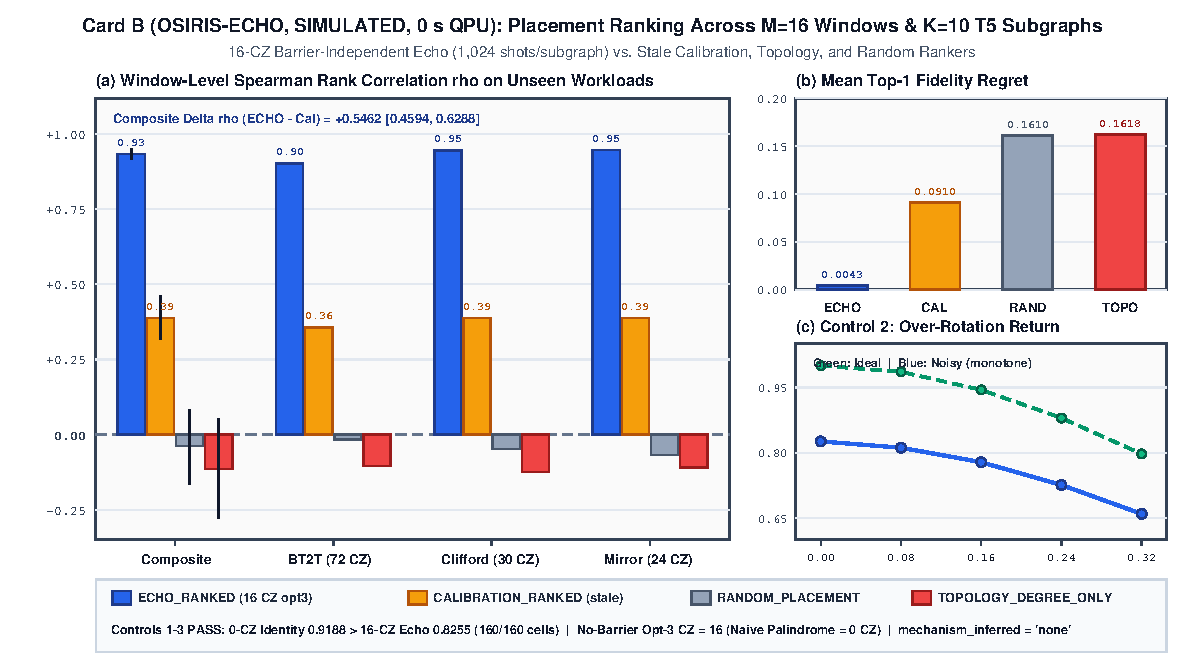
\includegraphics[width=\textwidth]{fig1_echo_placement_spearman_and_regret.pdf}
  \caption{\texttt{Card B} (\texttt{OSIRIS-ECHO}, \ecqExecTier, \ecqQpuSec\,s QPU) placement-ranking evaluation across $M = \ecqEchoWindowsM$ drifted calibration windows and $K = \ecqEchoPlacementsK$ candidate heavy-hex $T_5$ placements on \texttt{ibm\_fez} (\ecqEchoBootstrapB\ window-level bootstrap replicates). (a)~Window-level Spearman rank correlation $\bar{\rho}$ across composite and unseen \texttt{BT2T} (\ecqBtWorkloadCz\ \texttt{CZ}), random Clifford (\ecqCliffWorkloadCz\ \texttt{CZ}), and non-Clifford mirror (\ecqMirrorWorkloadCz\ \texttt{CZ}) circuits. (b)~Mean top-$1$ held-out fidelity regret relative to the per-window oracle placement. (c)~Control~2 monotone return decay under deliberate coherent over-rotation $\delta\theta \in [0, \ecqCtrlTwoMaxRad]$\,rad.}
  \label{fig:echo_spearman_regret}
\end{figure*}

\begin{table*}[t]
\caption{\texttt{Card B} (\texttt{OSIRIS-ECHO}) placement-ranking comparison across $M = \ecqEchoWindowsM$ calibration windows and $K = \ecqEchoPlacementsK$ candidate $T_5$ subgraphs (\ecqEchoTotalCells\ total window-subgraph cells; \ecqEchoShotsPerSubgraph\ probe shots per candidate; artifact SHA-256 prefix \ecqEchoRepSha).}
\label{tab:echo_ranking}
\begin{ruledtabular}
\begin{tabular}{lrrrrrrr}
Placement Ranker & Composite $\bar{\rho}$ ($95\%$ CI) & \texttt{BT2T} (\ecqBtWorkloadCz\ \texttt{CZ}) & Clifford (\ecqCliffWorkloadCz\ \texttt{CZ}) & Mirror (\ecqMirrorWorkloadCz\ \texttt{CZ}) & Top-$1$ Fid. & Top-$1$ Regret & Zero-Regret Win. \\
\hline
\ecqTableEchoRankingRows
\end{tabular}
\end{ruledtabular}
\end{table*}

\subsection{Out-of-Sample Ranking Transfer and Mandatory Controls}
Across $K = \ecqEchoPlacementsK$ disjoint or low-overlap $T_5$ subgraphs of the \ecqHeronQubits-qubit Heron~r2 lattice and $M = \ecqEchoWindowsM$ post-calibration drift windows (modeling realistic within-day coupler, readout, and coherent $\sqrt{X}$ over-rotation drift), each ranker selects placements using only pre-execution observables and is scored against exact held-out state fidelities on three unseen circuit classes: structured binary tetrahedral group inversion (\texttt{BT2T}, \ecqBtWorkloadCz\ \texttt{CZ}, depth \ecqBtWorkloadDepth), random five-qubit Clifford circuits (\ecqCliffWorkloadCz\ \texttt{CZ}, depth \ecqCliffWorkloadDepth), and stabilizer-twisted non-Clifford mirror circuits (\ecqMirrorWorkloadCz\ \texttt{CZ}, depth \ecqMirrorWorkloadDepth).

As summarized in Figure~\ref{fig:echo_spearman_regret} and Table~\ref{tab:echo_ranking}, \texttt{ECHO\_RANKED} achieves composite window-level Spearman $\bar{\rho} = +\ecqEchoSpearman$ ($95\%$ bootstrap CI $[+\ecqEchoSpearmanCiLo, +\ecqEchoSpearmanCiHi]$) versus $+\ecqCalSpearman$ ($[+\ecqCalSpearmanCiLo, +\ecqCalSpearmanCiHi]$) for \texttt{CALIBRATION\_RANKED}, $\ecqRandSpearman$ for \texttt{RANDOM\_PLACEMENT}, and $\ecqTopoSpearman$ for \texttt{TOPOLOGY\_DEGREE\_ONLY}, establishing a paired window-level gain $\Delta\bar{\rho} = +\ecqDeltaSpearman$ (two-sided $95\%$ CI $[+\ecqDeltaSpearmanCiLo, +\ecqDeltaSpearmanCiHi]$; one-sided lower confidence limit $+\ecqDeltaSpearmanOneSidedLcl > 0$). Ranking recovery transfers consistently across unseen \texttt{BT2T} ($\Delta\bar{\rho} = +\ecqBtDeltaSpearman$), Clifford ($+\ecqCliffDeltaSpearman$), and non-Clifford mirror ($+\ecqMirrorDeltaSpearman$) workloads, raising mean top-$1$ held-out fidelity from $\ecqCalTopOneFid$ to $\ecqEchoTopOneFid$ and reducing mean top-$1$ regret by $+\ecqRegretReductionPoint$ ($95\%$ CI $[+\ecqRegretReductionCiLo, +\ecqRegretReductionCiHi]$, a \ecqRegretRatioX\ reduction from $\ecqCalTopOneRegret$ to $\ecqEchoTopOneRegret$). All three mandatory falsifiers pass: Control~1 verifies $0$-\texttt{CZ} identity return ($\ecqCtrlOneIdentityReturn$) exceeds $\ecqEchoTotalCz$-\texttt{CZ} workload echo return ($\ecqCtrlOneEchoReturn$) in $\ecqCtrlOneCellsPassed / \ecqEchoTotalCells$ cells; Control~2 verifies strict monotone decay from $\ecqCtrlTwoNoisyStart$ to $\ecqCtrlTwoNoisyEnd$ (ideal $\ecqCtrlTwoIdealStart \to \ecqCtrlTwoIdealEnd$) across $\delta\theta \in [0, \ecqCtrlTwoMaxRad]$\,rad; and Control~3 confirms barrier-free non-cancellation (\ecqCardBVerdict).

\section{Card C (\texttt{OSIRIS-QEC}): Auditable Decoding and Four-Arm Crossing}

\subsection{Glass-Box Space-Time \texttt{MWPM} and Single-Fault Audits}
To ensure crossing verdicts are free of black-box decoder artifacts, \texttt{Card C} extracts an explicit circuit-level \texttt{SpaceTimeDEM} for both the five-qubit $[[3,1,3]]$ phase-flip repetition code and the seventeen-qubit Tomita--Svore~\cite{TomitaSvore2014} rotated $d = 3$ $[[9,1,3]]$ surface code (whose collision-free four-step \texttt{CNOT} schedule orients final check pairs perpendicular to the logical operators to prevent hook errors from halving fault distance). \texttt{AuditableMWPMDecoder} computes exact all-pairs Dijkstra shortest paths on the space-time defect graph and solves minimum-weight matching via exact $\mathcal{O}(k 2^k)$ bitmask dynamic programming for $k \le 16$ active defects and Edmonds' Blossom algorithm for $k > 16$, emitting a full matched-pair edge audit trail for every shot.

Exhaustive single-fault injection confirms \ecqSingleFaultRecoveryPct\ recovery (zero logical failures) across all \ecqSingleFaultLocRepZ\ $Z$-memory and \ecqSingleFaultLocRepX\ $X$-memory fault locations of $[[3,1,3]]$ and across all \ecqSingleFaultLocSurfZ\ $Z$-memory and \ecqSingleFaultLocSurfX\ $X$-memory fault locations of $[[9,1,3]]$. On $[[3,1,3]]$ at $R = 3$ ($\ecqMlNumSyndromes$ detector syndromes), \texttt{MWPM} agrees with an exact maximum-likelihood syndrome-coset table decoder on $\ecqMlAgreeCountX / \ecqMlNumSyndromes$ $X$-memory syndromes ($\ecqMlAgreeCountZ / \ecqMlNumSyndromes$ in $Z$-memory, matching \ecqSingleFaultRecoveryPct\ of single-fault syndromes) with $|\Delta P_{\mathrm{fail}}| = \ecqMlMwpmAbsDiffX$ ($\ecqMwpmDemPFailX$ versus $\ecqMlExactPFailX$), while the five-qubit Kraus density-matrix engine agrees with closed-form analytical $T_1/T_2$ plus coherent and SPAM evolution to $\le \ecqArmOneKrausMaxDiff$.

\subsection{Architectural Crossing Bifurcation Under Readout Drift}
At matched physical duration $T_{\mathrm{task}}(R) = R\,T_{\mathrm{round}}$ across $R \in \{1,2,3,5,7,9\}$, effective logical error per round and sustained crossing are defined by
\begin{align}
  \epsilon_L(R) &= \tfrac{1}{2}\Bigl[1 - \bigl(1 - 2 P_{\mathrm{fail}}(R)\bigr)^{1/R}\Bigr], \nonumber\\
  P_{\mathrm{fail}}(\mathrm{Arm\ 4}, R) &< \min\bigl\{P_{\mathrm{fail}}(\mathrm{Arm\ 1}, R),\, P_{\mathrm{fail}}(\mathrm{Arm\ 2}, R)\bigr\},
  \label{eq:eps_l_crossing}
\end{align}
evaluated across three noise regimes: \texttt{FEZ\_PUBLISHED} ($\epsilon_{\mathrm{CZ}} = \ecqFezCzErrPct$, $\epsilon_{\sqrt{X}} = \ecqFezSxErrPct$, $\epsilon_{\mathrm{RO}} = \ecqFezRoPubPct$, $\epsilon_{\mathrm{reset}} = \ecqFezResetPct$, $T_1 = \ecqFezToneUs\,\mu\mathrm{s}$, $T_2 = \ecqFezTtwoUs\,\mu\mathrm{s}$, $T_{\mathrm{round}} = \ecqFezTroundUs\,\mu\mathrm{s}$, $t_{\mathrm{ff}} = \ecqFezTffUs\,\mu\mathrm{s}$), \texttt{FEZ\_DRIFTED\_SPAM} ($\epsilon_{\mathrm{RO}} = \ecqFezRoDriftPct$ live SPAM staleness), and \texttt{H2\_1\_PUBLISHED} ($\epsilon_{\mathrm{ZZ}} = \ecqHtwoZzErrPct$, $\epsilon_{\mathrm{1Q}} = \ecqHtwoOneQErrPct$, $\epsilon_{\mathrm{RO}} = \ecqHtwoRoPct$, $\epsilon_{\mathrm{reset}} = \ecqHtwoResetPct$, $T_{\mathrm{round}} = \ecqHtwoTroundMs$\,ms, $t_{\mathrm{ff}} = \ecqHtwoTffMs$\,ms; \ecqRepShots\ shots/round on $[[3,1,3]]$, \ecqSurfShots\ shots/round on $[[9,1,3]]$).

\begin{table*}[t]
\caption{\texttt{Card C} (\texttt{OSIRIS-QEC}) four-arm logical error slope $\epsilon_L$ across $R \in \{1,2,3,5,7,9\}$ (artifact SHA-256 prefix \ecqQecRepSha). Postselected \texttt{Arm 3} conditional failure $P_{\mathrm{fail}}(R=9)$ and acceptance $A(R=9)$ are strictly isolated from unconditional \texttt{Arms 1}, \texttt{2}, \texttt{4a} (offline Pauli frame), and \texttt{4b} (physical feed-forward).}
\label{tab:cardc_crossing}
\begin{ruledtabular}
\begin{tabular}{llrrrrrrl}
Code & Target Profile & Arm 1 Bare & Arm 2 No-Corr & Arm 4a Frame & Arm 4b FF & $R_{\mathrm{cross}}$ (4a / 4b) & Arm 3 $R=9$ ($A$) & Verdict \\
\hline
\ecqTableCardCCrossingRows
\end{tabular}
\end{ruledtabular}
\end{table*}

\begin{figure*}[t]
  \centering
  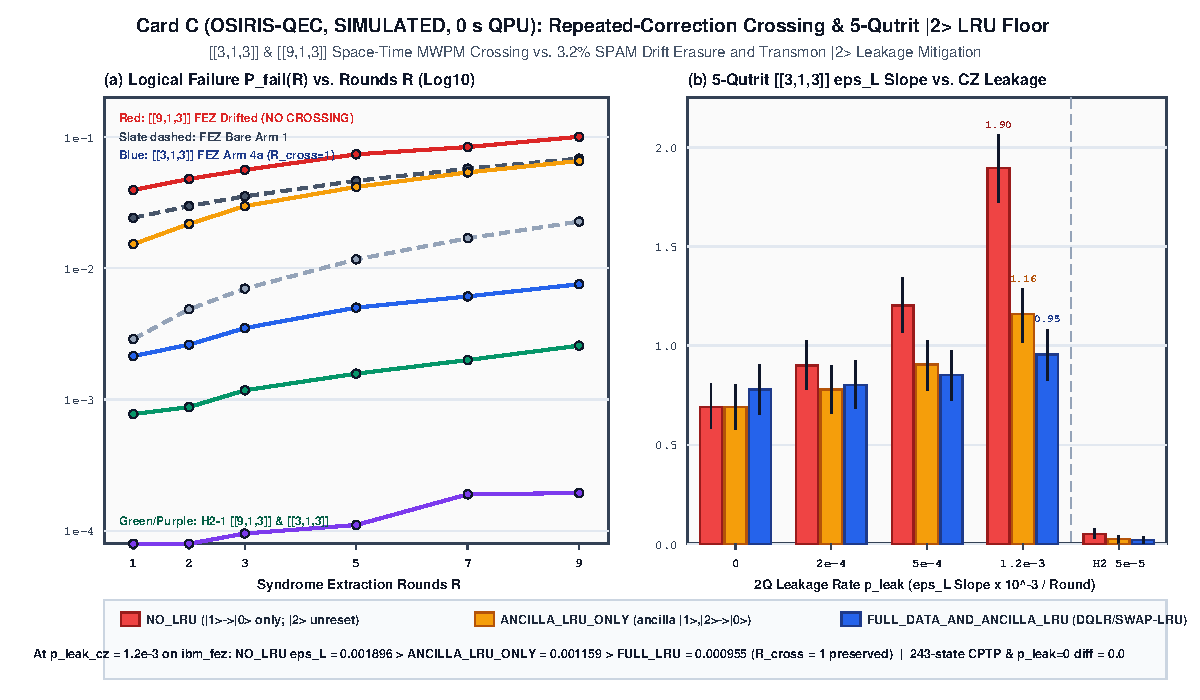
\includegraphics[width=\textwidth]{fig2_card_c_crossing_and_qutrit_lru.pdf}
  \caption{\texttt{Card C} (\texttt{OSIRIS-QEC}, \ecqExecTier, \ecqQpuSec\,s QPU) crossing trajectories and five-qutrit $|2\rangle$ \texttt{LRU} ablation. (a)~Unconditional $P_{\mathrm{fail}}(R)$ across $R \in \{1,2,3,5,7,9\}$: $[[3,1,3]]$ crosses at $R_{\mathrm{cross}} = 1$ across all regimes, whereas $\ecqFezRoDriftPct$ drifted readout on heavy-hex \texttt{ibm\_fez} erases the $[[9,1,3]]$ crossing above bare \texttt{Arm 1}, while native QCCD \texttt{H2-1} crosses cleanly at $R_{\mathrm{cross}} = \ecqHtwoSurfRCross$. (b)~Exact five-qutrit ($3^5 = \ecqQutritDim$-state) $[[3,1,3]]$ $\epsilon_L$ slope across \texttt{CZ} leakage rates comparing \texttt{NO\_LRU}, \texttt{ANCILLA\_LRU\_ONLY}, and \texttt{FULL\_DATA\_AND\_ANCILLA\_LRU} (\texttt{DQLR}/\texttt{SWAP-LRU}) plus \texttt{H2-1} ($p_{\mathrm{leak,ZZ}} = \ecqPLeakIon$).}
  \label{fig:cardc_crossing_lru}
\end{figure*}

Table~\ref{tab:cardc_crossing} and Figure~\ref{fig:cardc_crossing_lru}a reveal why pre-execution screening and native connectivity govern $d = 3$ break-even:
\begin{itemize}
  \item \emph{Native degree-two $[[3,1,3]]$ memory}: Embedding linearly without bridge SWAPs, offline Pauli-frame decoding (\texttt{Arm 4a}) crosses at $R_{\mathrm{cross}} = 1$ across all three profiles, suppressing $\epsilon_L$ by \ecqFezRepSuppX\ on \texttt{FEZ\_PUBLISHED} ($\ecqFezArmOneSlope \to \ecqFezRepArmFourASlope$; $P_{\mathrm{fail}}(R=9) = \ecqFezRepPFailRNine$ versus $\ecqFezArmOnePFailRNine$ bare) and by \ecqHtwoRepSuppX\ on \texttt{H2\_1\_PUBLISHED} ($\ecqHtwoArmOneSlope \to \ecqHtwoRepArmFourASlope$). Under $\ecqFezRoDriftPct$ drifted readout, \texttt{Arm 4a} rises to $\ecqDrfRepArmFourASlope$ and physical feed-forward (\texttt{Arm 4b}, $\ecqDrfRepArmFourBSlope$) delays crossing to $R_{\mathrm{cross}} = \ecqDrfRepRCrossFourB$.
  \item \emph{Degree-four $[[9,1,3]]$ rotated surface code}: Mapping degree-four plaquettes onto degree-three heavy-hex vertices incurs $+\ecqFezBridgeCz$ bridge \texttt{CZ} gates per round~\cite{ChamberlandHeavyHex2020}. Even on nominal \texttt{FEZ\_PUBLISHED}, \texttt{Arm 4a} ($\epsilon_L = \ecqFezSurfArmFourASlope$) barely crosses at $R_{\mathrm{cross}} = \ecqFezSurfRCrossFourA$ while physical feed-forward (\texttt{Arm 4b}, $\epsilon_L = \ecqFezSurfArmFourBSlope$) never beats bare \texttt{Arm 1}; under $\ecqFezRoDriftPct$ SPAM drift (\texttt{FEZ\_DRIFTED\_SPAM}), even \texttt{Arm 4a} degrades to $\epsilon_L = \ecqDrfSurfArmFourASlope$ ($P_{\mathrm{fail}}(R=9) = \ecqDrfSurfPFailRNine$), erasing the crossing completely (\texttt{STOP\_NO\_CROSSING\_AT\_TESTED\_ROUNDS}). By contrast, all-to-all QCCD \texttt{H2\_1\_PUBLISHED} incurs zero bridge SWAPs and crosses cleanly at $R_{\mathrm{cross}} = \ecqHtwoSurfRCross$ in both \texttt{Arm 4a} ($\ecqHtwoSurfArmFourASlope$) and \texttt{Arm 4b} ($\ecqHtwoSurfArmFourBSlope$). Meanwhile, postselected \texttt{Arm 3} attains low conditional error on drifted $[[9,1,3]]$ only by discarding $\ecqDrfSurfRejectRNinePct$ of runs by $R = 9$ ($A(9) = \ecqDrfSurfAccRNinePct$).
\end{itemize}

\section{Exact Five-Qutrit $|2\rangle$ Leakage and \texttt{LRU} Ablation}

\subsection{CPTP $\ecqQutritDim$-State Transmon and Hyperfine Leakage Model}
Two-level Pauli and Kraus models omit diabatic $|11\rangle \leftrightarrow |02\rangle / |20\rangle$ heating during transmon \texttt{CZ} gates~\cite{WoodGambetta2018,MiaoLeakage2023,MarquesLRU2023}. We close this evidence gap on $[[3,1,3]]$ by promoting each physical qubit to a qutrit in $\mathcal{H}_3 = \mathrm{span}\{|0\rangle,|1\rangle,|2\rangle\}$ ($\dim \mathcal{H}_3^{\otimes 5} = \ecqQutritDim$). For every native $(I_a \otimes H_d)\,\mathrm{CZ}_{a,d}\,(I_a \otimes H_d)$ check gate at gate-averaged leakage rate $p_{\mathrm{leak}}$ ($\lambda_{11} = 4 p_{\mathrm{leak}}$ on $|11\rangle$), the nine-dimensional CPTP channel combines computational evolution with diabatic heating and multi-round hook/spectator corruption:
\begin{align}
  K_{02} &= \sqrt{2 p_{\mathrm{leak}}}\,|0,2\rangle\langle 1,1|, \quad
  K_{20} = \sqrt{2 p_{\mathrm{leak}}}\,|2,+\rangle\langle 1,1|, \nonumber\\
  \mathcal{E}_{\mathrm{hook}}(\rho) &= \tfrac{1}{2}\rho + \tfrac{1}{2} Z_{\mathrm{partner}}\rho Z_{\mathrm{partner}}, \quad
  p_{\mathrm{seep}} = \frac{T_{\mathrm{round}}}{\tfrac{1}{2} T_1},
  \label{eq:qutrit_kraus}
\end{align}
where a leaked transmon in $|2\rangle$ fails to execute the computational $|11\rangle \mapsto -|11\rangle$ phase and injects persistent \ecqHookPhaseProbPct\ $Z$ phase/syndrome randomization onto its coupled partner across consecutive rounds until $|2\rangle$ seeps back to $|1\rangle$ ($p_{\mathrm{seep}} = \ecqFezSeepRoundPct$ per round on \texttt{ibm\_fez} due to bosonic enhancement $\Gamma_{2\to 1} = 2\Gamma_{1\to 0}$) or is actively reset, while dispersive binary readout classifies $|2\rangle$ as \texttt{'1'} with probability $\ecqPRoTwoAsOne$ (and \texttt{'0'} with $\ecqPRoTwoAsZero$). Because incoherent leakage and seepage preserve the single-qutrit algebra $\mathcal{B}(\mathbb{C}^2) \oplus \mathbb{R}|2\rangle\langle 2|$, the three-data-qutrit quantum instrument admits an exact $\ecqLiouvilleDim$-dimensional ($5^3 = \ecqLiouvilleDim$) real-Hermitian Liouville representation verified against full $\ecqQutritDim \times \ecqQutritDim$ density-matrix evolution to $\le \ecqQutritTwoFourThreeDiff$ (CPTP completeness error $\le \ecqQutritCptpMaxErr$) and matching the two-level \texttt{Card C} baseline with $\ecqZeroLeakDiff$ discrepancy across all three hardware profiles at $p_{\mathrm{leak}} = 0$.

\begin{table*}[t]
\caption{Exact five-qutrit ($3^5 = \ecqQutritDim$-state) $[[3,1,3]]$ logical error slope $\epsilon_L$ (with $\Delta\epsilon_L$ relative to the $p_{\mathrm{leak}} = 0$ \texttt{NO\_LRU} baseline), $R = 9$ consecutive $\ge 2$-round ancilla $|2\rangle$ streak fraction (\texttt{NO\_LRU} / \texttt{FULL\_LRU}), and $R = 9$ per-data-qutrit $|2\rangle$ occupancy (\texttt{NO\_LRU} / \texttt{FULL\_LRU}; artifact SHA-256 prefix \ecqLruRepSha).}
\label{tab:qutrit_lru}
\begin{ruledtabular}
\begin{tabular}{llrrrrrl}
Target Profile & $p_{\mathrm{leak}}$ & \texttt{NO\_LRU} $\epsilon_L$ ($\Delta\epsilon_L$) & \texttt{ANCILLA\_LRU} $\epsilon_L$ ($\Delta\epsilon_L$) & \texttt{FULL\_LRU} $\epsilon_L$ ($\Delta\epsilon_L$) & Anc.\ Streak $R=9$ & Data $P(|2\rangle)$ $R=9$ & Crossing \\
\hline
\ecqTableQutritLruRows
\end{tabular}
\end{ruledtabular}
\end{table*}

\subsection{Comparison of \texttt{NO\_LRU}, \texttt{ANCILLA\_LRU\_ONLY}, and \texttt{FULL\_DATA\_AND\_ANCILLA\_LRU}}
We compare three reset/mitigation architectures across $p_{\mathrm{leak,CZ}} \in \{0, \ecqPLeakLow, \ecqPLeakMid, \ecqPLeakHigh\}$ on \texttt{ibm\_fez} and $p_{\mathrm{leak,ZZ}} = \ecqPLeakIon$ on \texttt{H2-1} (Table~\ref{tab:qutrit_lru} and Figure~\ref{fig:cardc_crossing_lru}b):
\begin{enumerate}
  \item \texttt{NO\_LRU} (computational $|1\rangle \to |0\rangle$ reset leaving $|2\rangle$ unreset): At $p_{\mathrm{leak,CZ}} = \ecqPLeakHigh$ on \texttt{FEZ\_PUBLISHED}, $\ecqLruNoHighStreakPct$ of $R = 9$ trajectories suffer $\ge 2$-round consecutive ancilla $|2\rangle$ streaks. Because a leaked ancilla couples to two data qubits per round while outputting \texttt{'1'} at rate $\ecqPRoTwoAsOne$ ($1 \oplus 1 = 0$ silent detector streaks), space-time hook errors reduce effective fault distance and bend $\epsilon_L(R)$ upward from $\ecqLruNoHighEpsRThree$ ($R = 3$) to $\ecqLruNoHighEpsRNine$ ($R = 9$, $P_{\mathrm{fail}}(9) = \ecqLruNoHighPFailRNine$), inflating fitted $\epsilon_L$ by \ecqLruNoHighInflX\ to $\ecqLruNoHighSlope$ ($95\%$ CI $[\ecqLruNoHighCiLo, \ecqLruNoHighCiHi]$, $\Delta\epsilon_L = +\ecqLruNoHighDelta$).
  \item \texttt{ANCILLA\_LRU\_ONLY} (unconditional multi-level $|1\rangle,|2\rangle \to |0\rangle$ ancilla reset each round, infidelity $\ecqTransmonAncLruInfid$): Eliminates multi-round ancilla $|2\rangle$ streaks ($\ecqLruAncHighStreakPct$) and lowers $\epsilon_L$ at $p_{\mathrm{leak,CZ}} = \ecqPLeakHigh$ to $\ecqLruAncHighSlope$ ($95\%$ CI $[\ecqLruAncHighCiLo, \ecqLruAncHighCiHi]$, $\Delta\epsilon_L = +\ecqLruAncHighDelta$), outperforming \texttt{NO\_LRU} already at $p_{\mathrm{leak,CZ}} = \ecqPLeakLow$ ($\ecqLruAncLowSlope$ versus $\ecqLruNoLowSlope$). However, unreset data-qutrit $|2\rangle$ population still accumulates to $\ecqLruAncHighDataLeakPct$ per data transmon by $R = 9$ ($\ecqLruNoHighDataLeakPct$ under \texttt{NO\_LRU}).
  \item \texttt{FULL\_DATA\_AND\_ANCILLA\_LRU} (\texttt{DQLR}/\texttt{SWAP-LRU}: multi-level ancilla reset plus every-round data $|2\rangle \to |1\rangle$ seepage pulse~\cite{MiaoLeakage2023,MarquesLRU2023} with 1Q gate overhead $\ecqTransmonDqlrOneQErr$ and $\ecqTransmonDqlrDurNs$\,ns duration): At $p_{\mathrm{leak,CZ}} = 0$, the \texttt{DQLR} pulse incurs a transparent $+\ecqLruFullZeroOverhead$ baseline cost ($\epsilon_L = \ecqLruFullZeroSlope$), crossing below \texttt{ANCILLA\_LRU\_ONLY} by $p_{\mathrm{leak,CZ}} = \ecqPLeakMid$ ($\ecqLruFullMidSlope$ versus $\ecqLruAncMidSlope$ and $\ecqLruNoMidSlope$). At $p_{\mathrm{leak,CZ}} = \ecqPLeakHigh$, \texttt{FULL\_DATA\_AND\_ANCILLA\_LRU} pins steady-state data $|2\rangle$ occupancy to $\ecqLruFullHighDataLeakSci$ across all rounds, restores monotone per-round suppression ($\epsilon_L(9) = \ecqLruFullHighEpsRNine$, $P_{\mathrm{fail}}(9) = \ecqLruFullHighPFailRNine$), and suppresses $\epsilon_L$ to $\ecqLruFullHighSlope$ ($95\%$ CI $[\ecqLruFullHighCiLo, \ecqLruFullHighCiHi]$, $\Delta\epsilon_L = +\ecqLruFullHighDelta$), eliminating \ecqLruPenaltyMitPct\ of the unmitigated leakage penalty and preserving $R_{\mathrm{cross}} = 1$ even under combined $\ecqFezRoDriftPct$ readout drift ($\ecqDrfFullHighSlope$ versus $\ecqDrfAncHighSlope$ and $\ecqDrfNoHighSlope$).
\end{enumerate}
On trapped-ion \texttt{H2\_1\_PUBLISHED} ($p_{\mathrm{leak,ZZ}} = \ecqPLeakIon$ spontaneous Raman scattering), unpumped Zeeman leakage would raise $\epsilon_L$ from $\ecqHtwoRepArmFourASlope$ to $\ecqHtwoLruNoSlope$ ($\Delta\epsilon_L = +\ecqHtwoLruNoDelta$), whereas optical-pumping ancilla reset ($\ecqHtwoLruAncSlope$) and data repumping ($\ecqHtwoLruFullSlope$) restore the leakage-free QCCD floor.

\section{Conclusion and Scope Limitations}
Unifying \texttt{Card B} (\texttt{OSIRIS-ECHO}) and \texttt{Card C} (\texttt{OSIRIS-QEC}) establishes clear quantitative preconditions for hardware QEC execution: on sparse heavy-hex superconducting lattices, $\ecqEchoNoBarrierOptThreeCz$-\texttt{CZ} stabilizer-reflected echo screening (\ecqRegretRatioX\ top-$1$ regret reduction) and full ancilla-plus-data \texttt{LRU} reset ($\epsilon_L = \ecqLruFullHighSlope$ at $p_{\mathrm{leak,CZ}} = \ecqPLeakHigh$) jointly protect $[[3,1,3]]$ crossing ($R_{\mathrm{cross}} = 1$), whereas $[[9,1,3]]$ surface-code memory should target native all-to-all QCCD architectures ($R_{\mathrm{cross}} = \ecqHtwoSurfRCross$, $\epsilon_L = \ecqHtwoSurfArmFourBSlope$ with feed-forward) until heavy-hex readout drift and bridge-SWAP overheads are reduced. All results here are strictly \ecqExecTier\ (\texttt{provider\_job\_id}: \ecqJobId, \ecqQpuSec\,s QPU), echo ranking infers no microscopic error mechanism (\texttt{mechanism\_inferred} = \texttt{none}), and $d = 3$ crossing results do not constitute evidence of multi-distance ($d = 3 \to 5 \to 7$) fault-tolerant scaling.

\section*{Data and Code Availability}
Audited simulation gates (\ecqEchoPySha, \ecqQecPySha, \ecqLruPySha), deterministic JSON reports (\ecqEchoRepSha, \ecqQecRepSha, \ecqLruRepSha), and the RFC~8785 JCS reproducibility capsule (\ecqCapsuleSha) are archived under \texttt{experiments/echo\_placement/}, \texttt{experiments/qec\_card\_c/}, and \texttt{papers/echo\_and\_card\_c\_qec\_gates/}.

\begin{thebibliography}{9}
\bibitem{GoogleSurface2023} Google Quantum AI, Nature \textbf{614}, 676 (2023).
\bibitem{MiaoLeakage2023} K. C. Miao \emph{et al.} (Google Quantum AI), Nat. Phys. \textbf{19}, 1780 (2023).
\bibitem{ChamberlandHeavyHex2020} C. Chamberland, G. Zhu, T. J. Yoder, J. B. Hertzberg, and A. W. Cross, Phys. Rev. X \textbf{10}, 011022 (2020).
\bibitem{QuantinuumLogical2024} M. P. da Silva \emph{et al.}, arXiv:2404.02280 (2024).
\bibitem{DavisRO0607Zenodo2026} D. P. Davis, \emph{Transient Readout Staleness and Multiplexed Isolation on 156-Qubit IBM Heron r2 Processors (RO-06/RO-07)}, Zenodo (2026), \texttt{doi:10.5281/zenodo.24420902}.
\bibitem{DavisTMAP02Zenodo2026} D. P. Davis, \emph{Calibration-Ranked Layout Sensitivity and Sign Reversal on Superconducting Heavy-Hex Processors (TMAP-02)}, Zenodo (2026), \texttt{doi:10.5281/zenodo.24406426}.
\bibitem{TomitaSvore2014} Y. Tomita and K. M. Svore, Phys. Rev. A \textbf{90}, 062320 (2014).
\bibitem{WoodGambetta2018} C. J. Wood and J. M. Gambetta, Phys. Rev. A \textbf{97}, 032306 (2018).
\bibitem{MarquesLRU2023} J. F. Marques \emph{et al.}, Phys. Rev. Lett. \textbf{130}, 250602 (2023).
\end{thebibliography}

\end{document}
